\section{Experiments and Results}
\label{sec:experiments}
Our experiments are focused on sentence classification task. %where the task is to assign a label to a given sentence. 
%\subsection{Experimental Setup}
%These numbers might be different in other frameworks but should have similar trends.
\subsection{Datasets:} %\\
For all the experiments reported we have used the following two sentence classification datasets:    \\
%\subsubsection{Movie Review Dataset (MR)}
%The Movie Review dataset~\cite{maas2011learning} is a common benchmark classification dataset that contains movie reviews, that should be classified as either positive or negative. On an average the reviews are about 200 words long. It has balanced train and test sets containing 25k examples each.
\textbf{Stanford Sentiment Treebank (SST2)}
SST2 ~\cite{socher2013recursive} is a common text classification benchmark dataset that contains movie reviews, to be classified according to their sentiment. On an average the reviews are about 200 words long. The dataset contains standard train, dev, test splits and binary sentiment labels. \\
\textbf{Books Intent Classification Dataset}
We use a proprietary dataset of around 60k annotated utterances of users interacting with a popular digital assistant about books related functionality. Each utterance is manually labeled with the user intent e.g., search for a book, read a book and others, with the task being to predict the user intent from a set of 20 intents. We choose 50k utterances as our training data, 5k as test data and 5k as dev data.%\\ \\
\subsection{Models:}%\\
We evaluate our compression strategy on two types of widely used neural models: \\ %which are commonly used for classification tasks:\\
\textbf {Long Short Term Memory(LSTM)}
LSTMs, are powerful and popular sequential models
for classification tasks. The LSTM units are recurrent inn nature, designed to
handle long term dependencies through the use of input, output
and forget gates and a memory cell. For input $X=x_1,
\cdots x_T $ and corresponding word embedding input vectors $e_i, i=1, \cdots
T$, LSTM computes a representation $r_t$ at each word $t$, which is denoted as
$r_t = \phi ( e_t ,r_{t-1} )$. Here, for sentence classification, we used the representation obtained from the final timestep of the LSTM and
pass it through a softmax for classification:
%\begin{gather}
$r^{sent} = r^{forw}_{T},$ and $ \hat{S}=softmax( W_{s} r^{sent} + b_{s}) $
%\end{gather}
where $r^{sent}$ is the sentence representation, and $\hat{S}$ is the label
predicted. In our experiments with LSTM, we used
300-dimensional Glove embeddings to initialize the embedding layer for all the methods, e.g., baselines 1, 2 and our proposed compression method. Our vocabulary size $V$ contains only the words that appear in the training data, and we compress the input word embedding matrix $W$ (original size $V \times 300$).\\
\textbf{Deep Averaging Network (DAN)} DAN is a
bag-of-words neural model that averages the word embeddings in each input
utterance to create a sentence representation $r^{sent}$ that is passed
through a series of fully connected layers, and fed into a softmax layer for
classification. Assume an input sentence $X$ of length $T$ and
corresponding word embeddings $e_i$, then the sentence representation is: $r^{sent} = \frac{1}{T} \sum_{i=1}^T { e_i }$
%\begin{gather}
%r^{sent} = \frac{1}{T} \sum_{i=1}^T { e_i }
%\end{gather}
%DAN has been proven a state-of-the-art model for simple classification tasks
%such as the Factoid Question Answering task~\cite{iyyer2015deep}. 
In our setup, we have two fully connected layers after the sentence representation $r^{sent}$,
of sizes 1024 and 512 respectively. For the DAN experiments we used the DAN-RAND
~\cite{iyyer2015deep} variant where we take a randomly initialized 300
dimensional embedding. To make the comparison fair, all experiments with DAN models, including quantization (baseline 1), the offline compression method (baseline 2) and the proposed compression method are done using randomly initialized word embedding matrices. For example, our baseline 2 is to use appropriate low-rank randomly initialized embedding matrix. %\\ \\
\subsection{Experimental Setup}%\\
Our experiments are performed on 1 Tesla K80 GPU, using SGD optimizer with CALR policy (Sec.\ref{subsec:method_training_scheme}), initial learning rate upper bound of 0.001. We use dropout of 0.4 between layers and L2 regularization with weight of 0.005. Our metrics include accuracy and model size. Accuracy is simply the fraction of utterances with correctly predicted label. The model size is calculated as sum of (.data + .index + .meta) files stored by tensorflow. 
%Setting up the experiments with randomly initialized embeddings for DAN, as well as GloVe
%initialized ensures that all the gains we report is not due to low dimensional
%latent structure of the initialization embedding matrix but are attributed to
%our proposed approach.
\begin{table}[b]
  \centering
  \scalebox{0.9}{
	\begin{tabular}{lllll} \hline
		Model & LR Schedule & Acc.\\ \hline
		\multicolumn{3}{c}{Uncompressed LSTM Model}\\ \hline
		\citeauthor{tai2015improved}&    AdaGrad       & 84.90  \\
		\citeauthor{smith2017cyclical}& CLR & 84.71\\
		Ours & CALR & \textbf{86.03}\\\hline
		\multicolumn{3}{c}{Uncompressed DAN-RAND Model}\\ \hline
		\citeauthor{iyyer2015deep} &    AdaGrad       & 83.20  \\
		\citeauthor{smith2017cyclical} & CLR & 83.84\\
		Ours & CALR & \textbf{84.61}		
	\end{tabular} }
	\caption{\small Comparison of initial Uncompressed Model for different Learning Rate Schedules on SST2}
	\label{results:uncompressed}	
\end{table}

\subsection{Results on Uncompressed Models}
\label{sec:experiments_uncompresed}
To effectively train our uncompressed benchmark networks we experimented with
different adaptive learning rate schedules. Table~\ref{results:uncompressed}
emperically demonstrates the effectiveness of our proposed learning rate update
policy (CALR) on the SST2 test set. For both the
models CALR outperforms the corresponding state-of-the-art sentence
classification accuracy reported in the literature. For LSTM we improve the
accuracy from 84.9\%~\cite{socher2013recursive} to 86.03\% (1.33\% relative
improvement) whereas on DAN-RAND we are able to improve from 83.2\%
~\cite{iyyer2015deep} to 84.61\% (1.7\% relative improvement). We also report
results on training the network with CLR without our cyclic annealing. For both
DAN-RAND and LSTM, CLR achieves performance that is similar to the previously reported state-of-the-art. The proposed CALR outperforms CLR, which supports the effectiveness of the proposed CALR policy.
%which further strenghthens the effectiveness of CALR policy.

\begin{table}[t]
  \centering
  \scalebox{0.9}{
        \begin{tabular}{lllll} \hline
Model               & R(\%) & Size(MB)    &  Acc. & Acc.\\ \hline
\multicolumn{5}{c}{Uncompressed LSTM  model}\\ \hline
LSTM          & 0             & \bf{53.25} & \bf{86.03}            & -     \\
\hline
\multicolumn{5}{c}{Quantized model (Baseline 1) }\\ \hline
16 bit  & 50            & 30.16 & 85.08              & -        \\
8 bit & 75            & 18.21 & 85.01              & -       \\ \hline 
\multicolumn{5}{c}{SVD: Proposed vs Offline Compression (Baseline 2)}\\\hline
                &               &          &   Proposed   &   Baseline2  \\ 
LSTM            & 10            & 48.66 & 85.72              & 85.45    \\
            & 30            & 38.52 & 85.68              & 84.95     \\
          & 50            & 28.45 & 85.67              & 84.24     \\
          & 70            & 18.38 & 85.45              & 83.09     \\
         & 90            & \bf{6.94}  & \bf{85.11}              & 82.54      \\ \hline\hline
\multicolumn{5}{c}{Uncompressed DAN model}\\\hline
DAN             & 0             & \bf{52.84}  & \bf{84.61}            & -    \\  \hline
\multicolumn{5}{c}{Quantized model (Baseline 1) }\\ \hline
16 bit & 50            & 28.36 & 83.18              & -            \\
8 bit & 75            & 18.13 & 82.94              & -             \\ \hline
\multicolumn{5}{c}{SVD: Proposed vs Offline Compression (Baseline 2)}\\ \hline
             &               &          &   Proposed   &   Baseline2  \\ 
DAN             & 10            & 47.29 & 84.24              & 83.47      \\
                    & 30            & 37.23 & 83.83         & 83.31     \\
                    & 50            & 27.16 & 83.72         & 82.87       \\
                    & 70            & 17.18 & 83.67          & 82.86     \\
                    & 90            & \bf{6.21}  & \bf{83.11}          & 82.59  \\ \hline
\end{tabular}}
	\caption{\small Compression and accuracy results on SST2 dataset. R(\%) refers to percentage of model size reduction, Size is the model size, and Acc is the classification accuracy. All DAN models use the DAN-RAND variant.}
	\label{results:sst}
\end{table}


\begin{table}[t]
  \centering
  \scalebox{0.9}{
	\begin{tabular}{lllll} \hline
		Model               & R(\%) & Size(MB)    &  Acc. & Acc.\\ \hline
		\multicolumn{5}{c}{Uncompressed LSTM model}\\ \hline
		LSTM          & 0             &\bf{29.34} & \bf{91.78}            & -     \\
		\hline
		\multicolumn{5}{c}{Quantized model (Baseline 1) }\\ \hline
		16 bit  & 50            & 17.92  & 90.16             & -        \\
		8 bit & 75            & 10.05  & 89.96              & -       \\ \hline 
		\multicolumn{5}{c}{SVD: Proposed vs Offline Compression (Baseline 2)}\\\hline
		&               &          &   Proposed   &   Baseline2  \\ 
		LSTM            & 10          & 26.76 & 91.71          & 91.07    \\
		& 30            & 21.69 & 91.63            & 90.97     \\
		& 50            & 16.62 & 91.54             & 90.87     \\
		& 70            & 10.31  &91.47              & 90.58     \\
		& 90            & \bf{4.89}  &\bf{90.94}              &89.83      \\ \hline\hline
		\multicolumn{5}{c}{Uncompressed DAN model}\\\hline
		DAN             & 0             & \bf{37.03} & \bf{90.18}            & -    \\  \hline
		\multicolumn{5}{c}{Quantized model (Baseline 1) }\\ \hline
		16 bit & 50            & 25.68  & 89.38              & -            \\
		8 bit & 75            & 16.41  & 88.86           & -             \\ \hline
		\multicolumn{5}{c}{SVD: Proposed vs Offline Compression (Baseline 2)}\\ \hline
		&               &          &   Proposed   &   Baseline2  \\ 
		DAN             & 10            & \bf{33.96}  & \bf{90.15}              & 87.35     \\
		& 30            & 29.43  & 90.12         & 87.34     \\
		& 50            & 23.16  & 89.47         & 87.14       \\
		& 70            & 18.21 & 89.55         & 86.15     \\
		& 90            & \bf{13.08}  & \bf{89.23}          & 83.72  \\ \hline
	\end{tabular}}
	\caption{\small Compression and accuracy results on the Books Intent dataset. R(\%) refers to percentage of model size reduction, Size is the model size, and Acc is the classification accuracy. All DAN models use the DAN-RAND variant.}
	\label{results:intent}
\end{table}


\subsection{Results on SST2 }
Table~\ref{results:sst} shows compression and accuracy results on the SST2 test dataset
for our proposed methods, the two baselines described in Section
~\ref{subsec:method_baselines}, and for two types of models: LSTM~(upper table
rows) and DAN-RAND~(lower table rows). For both types of models, we first report the
original uncompressed model size and accuracy.  For the quantization baseline
(baseline 1), we report size and accuracy numbers for 8-bit and 16-bit
quantization. For the SVD-based methods, both for the offline embedding
compression (baseline 2) and our proposed compression method, we compare size
and accuracy for different percentages of model size reduction $R$, where $R=1-p$. This reduction
corresponds to different fractions $p$ and to different number of selected singular values
$k$ (Section \ref{sec:method_svd}).

%Specifically, for LSTM the uncompressed model achieves $86.03$ accuracy which is state-of-the-art for this task and this model \cite{tai2015improved}. We can make similar observations for the DAN-RAND model, where the uncompressed model achieves $84.61$ accuracy which is higher than state of the art for this task and this model (\cite{iyyer2015deep} used DAN-RAND on SST2 and achieved $83.2$). 

From Table~\ref{results:sst}, we observe that our proposed compression method
outperforms both baselines for both types of models. For LSTM, our method achieves
$R=90\%$ compression with $85.11$ accuracy e.g., only 1\% rel. degradation
compared to the uncompressed model, while the offline embedding compression
(baseline 2) achieves $82.54$ (4\% rel degradation vs uncompressed). Looking at
$R=50\%$ our method achieves accuracy of $85.67$ (0.4\% rel degradation) vs
$84.24$ for baseline 2 (2\% rel degradation) and $85.08$ for baseline 1 which
does 16-bit compression (1\% rel degradation).  For DAN-RAND and for $R=90\%$ compression, our method achieves accuracy of $83.11$ which corresponds to 1.7\% rel
degradation vs an uncompressed model, and outperforms baseline 2 that has
accuracy of $82.59$ (2.4\% rel. degradation). Similar trends are seen across
various size reduction percentages $R$. \\
Comparing LSTM vs DAN-RAND models in terms of the gain we achieve over quantization, we observe that for LSTM our compression outperforms quantization by a large margin for the same compression rates, while for DAN-RAND the gain is less pronounced. We hypothesize that this is because LSTMs have recurrent connections and a larger number of low precision multiplications compared to DAN, which has been shown to lead to worse performance\cite{lin2015neural}. Thus, we expect our method to benefit the most over quantization when the network is deep.

% \begin{figure*}[t]
%        \centering
%         \begin{subfigure}[b]{0.45\textwidth}
%                 \centering
%                 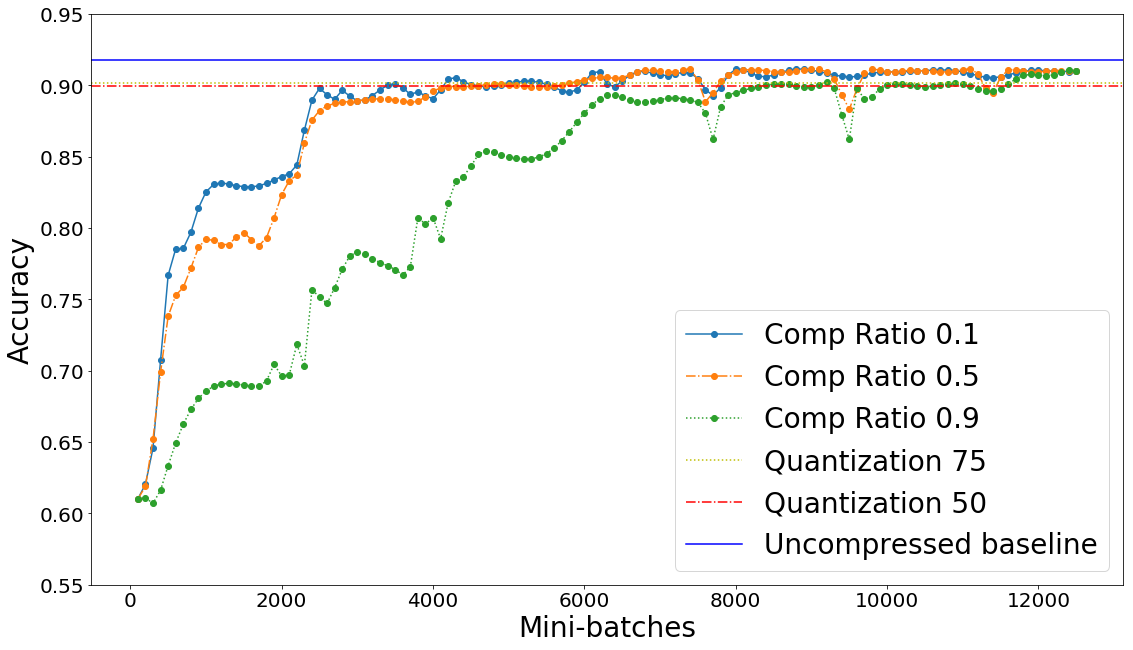
\includegraphics[width=\linewidth]{alexa_lstm.png}
%                 \caption{LSTM model}
%                 \label{fig:lstm_alexa}
%         \end{subfigure}%
%         \begin{subfigure}[b]{0.45\textwidth}
%                 \centering
%                 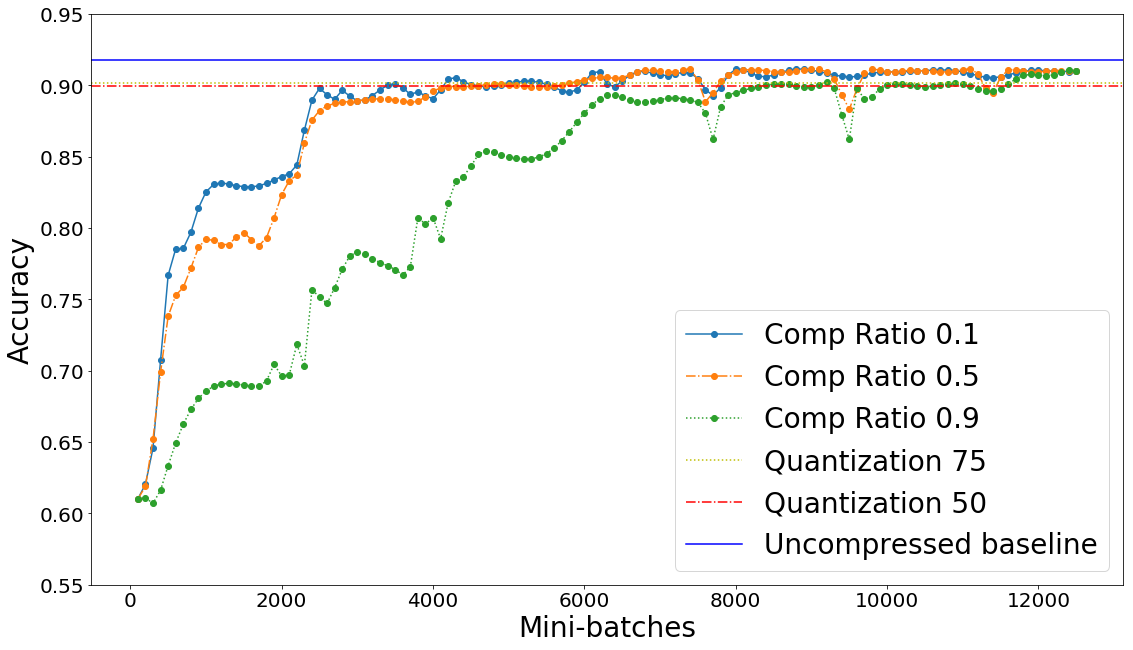
\includegraphics[width=\linewidth]{alexa_lstm.png}
%                 \caption{DAN model}
%                 \label{fig:dan_alexa}
%         \end{subfigure}%
%         \caption{Dev set accuracy vs training mini batches for various compression percentages R for the Books Intent dataset.}
%         \label{fig:alexa_plots}
% \end{figure*}
\begin{figure*}[]
	\centering
	\begin{subfigure}[b]{0.45\textwidth}
		\centering
		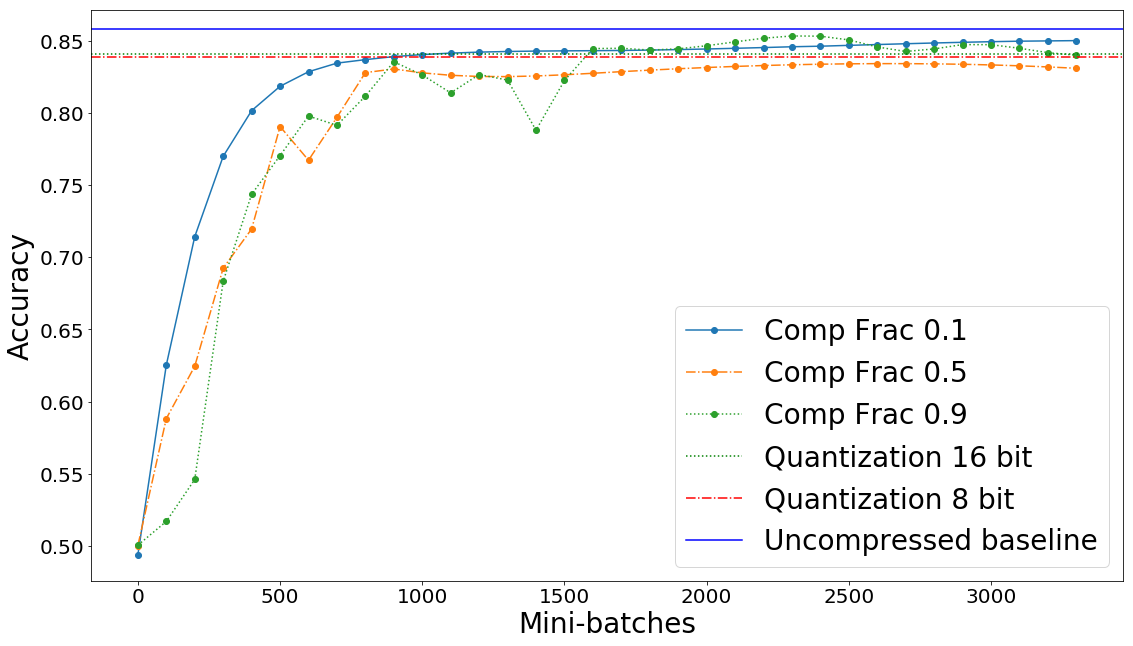
\includegraphics[width=\linewidth]{sst_lstm.png}
		\caption{LSTM model}
		\label{fig:lstm_sst2}
	\end{subfigure}%
	\begin{subfigure}[b]{0.45\textwidth}
		\centering
		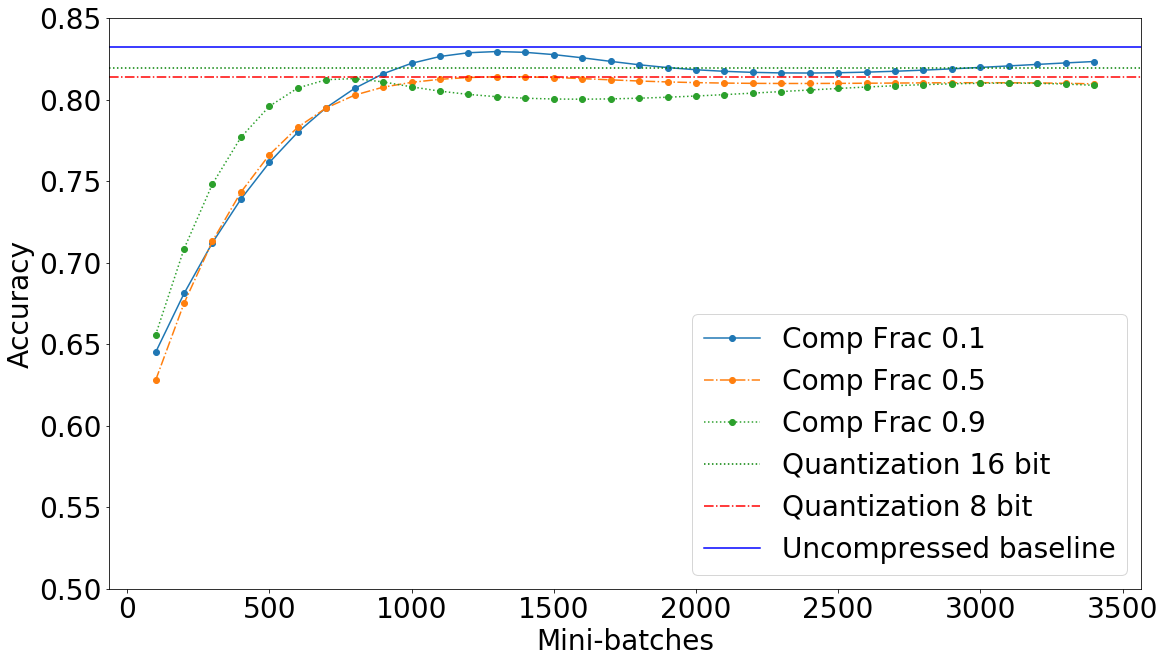
\includegraphics[width=\linewidth]{sst_dan.png}
		\caption{DAN-RAND model}
		\label{fig:dan_sst2}
	\end{subfigure}%
	\caption{\small Dev set accuracy vs training mini batches for various compression percentages R for the SST2 dataset}
	\label{fig:sst2_plots}
\end{figure*}

To illustrate how our proposed method benefits from re-training the model after
compressing the embedding input matrix, in Fig~\ref{fig:sst2_plots} we plot the
dev set accuracy for SST2 across training mini-batches for different compression
percentages R and for both LSTM and DAN-RAND. For comparison, we plot the dev
accuracy of 8-bit and 16-bit quantization (baseline 1) that remains stable
across epochs as the quantized model is not retrained after compression. As a
further comparison, we plot the uncompressed model accuracy on the dev which is
kept stable as well (we assume this as our benchmark point). We observe that,
while our compressed model starts off at a lower accuracy compared to both the
uncompressed model and the quantization baseline, it rapidly improves with
training and stabilizes at an accuracy that is higher than the quantization
method and comparable to the original uncompressed model. This indicates that
re-training after SVD compression enables us to fine-tune the layer parameters
$W_a$ and $W_b$ towards the target task, and allows us to recover most of the
accuracy.

\vspace{-1mm}
\subsection{Results on Books Intent Dataset}
Table~\ref{results:intent} shows compression and accuracy results on the
proprietary Books Intent test set for our proposed methods vs the two baselines,
for the LSTM and DAN-RAND models. Overall, we make similar observations as for
the SST2 dataset. Our proposed method achieves better accuracy across
compression percentages compared to both offline embedding compression and
quantization for both LSTM and DAN-RAND. For example, for LSTM and R=90\% compression we
achieve accuracy of 90.94\% which corresponds to 1\% degradation compared to the
uncompressed model, while offline embedding compression (baseline 2) achieves
accuracy of 89.83 (2\% degradation). We also examined the plots of dev set
accuracy while re-training the proposed compressed model across mini-batches and
observed similar trends as for SST2 (plots are omitted for brevity).

\vspace{-1mm}
\subsection{Results on Inference Time}
%We don't include the development accuracy tuning plots but we observe similar trends as the SST dataset. 
In Table~\ref{results:time_analysis}, for both LSTM and DAN-RAND, we report inference times for the SST2 test set for different compression fractions using the proposed compression vs inference times for 16-bit and 8-bit fixed point quantization~(baseline 2). As expected, for our method we see a decrease in inference time as the compression fraction~(R) increases. We observe similar trends for the quantization method, where 8-bit is faster
than 16-bit. For similar compression rates~(16-bit equivalent to 50\%
compression and 8-bit is equivalent to 75\% compression) our method and baseline 2 (fixed-point-quantization) show similar inference times. Therefore, our method does not introduce any significant latency during inference while regaining the accuracy. 
\begin{table}[]
  \centering
  \scalebox{0.9}{
	\begin{tabular}{lllll} \hline
		& LSTM && DAN-RAND \\ \hline
		R(\%) & Proposed & Baseline 2 &  Proposed & Baseline 2\\ \hline 
		10 &  10.71 & -. & 1.38 & -  \\
		50 & 9.28 & 9.23 & 0.89 & 0.93\\
		70 & 9.21 & -. & 0.62 & -\\
		75 & 9.11 &  9.08 & 0.59 & 0.62\\
		90 & 8.46 & - & 0.45 & -\\		\hline	
	\end{tabular}	}
	\caption{\small Inference Time on the SST2 test set (seconds)}
	\label{results:time_analysis}
\end{table}

%We observe similar trends on both of our experiment settings we note a number of things
%\begin{enumerate}
%	\item By doing spectral decomposition we observe that we start lower then quantization in terms of accuracy but we recover the same on fine tuning, acheiving very close performance to the baseline
%	\item Training a new network from scratch with a similar architecture we are unable to the same accuracy as the fine tuned network after compression.
%\end{enumerate}



% \begin{table*}[]
% 	%% \vspace{-3.0cm}
% 	\centering
% 	\caption{Compression results on books dataset}
% 	\label{results:intent}
%         \begin{tabular}{lllll}
% MODEL               & Reduction(\%) & SIZE*(MB) &  Base Accuracy & \\ \hline
% LSTM (100)          & 0             & 29.34 MB & 91.78         & -          \\
% 16 Bit Fixed Point  & 50            & 17.92 MB & 90.16         & -             \\
% 8   Bit Fixed Point & 75            & 10.05 MB & 89.96         & -             \\ \hline \hline
%                     &               &          &   Acc {[}Proposed{]}   &   Acc {[}BaseLine2{]}  \\ 
% LSTM LRC            & 10            & 26.76 MB & 91.71         & 91.07          \\
%                     & 30            & 21.69 MB & 91.63         & 90.97          \\
%                     & 50            & 16.62 MB & 91.54         & 90.87          \\
%                     & 70            & 10.31 MB & 91.47         & 90.58          \\
%                     & 90            & 4.89 MB  & 90.94         & 89.83          \\ \hline
%                     &               &          &               &                \\ \hline \hline
%                     &               &          &  Base Accuracy             &                \\ 
% DAN                 & 0             & 37 MB    & 90.18         & -          \\
% 16 Bit Fixed Point  & 50            & 25.68 MB & 89.38         & -             \\
% 8   Bit Fixed Point & 75            & 16.41 MB & 88.86         & -            \\ \hline \hline
%                     &               &          &   Acc {[}Proposed{]}   &   Acc {[}BaseLine2{]}  \\ 
% DAN LRC              & 10            & 34 MB    & 90.15         & 87.35          \\
%                     & 30            & 29 MB    & 90.12         & 87.34          \\
%                     & 50            & 23 MB    & 89.47         & 87.14          \\
%                     & 70            & 18 MB    & 89.55         & 86.15          \\
%                     & 90            & 13 MB    & 89.23         & 83.72          \\ 
% \end{tabular}
% \end{table*}






%\begin{figure*}[htbp]
%	%% \vspace{-0.9cm}
%	\begin{minipage}{\textwidth}
%		\begin{minipage}[b]{0.54\textwidth}
%			\centering 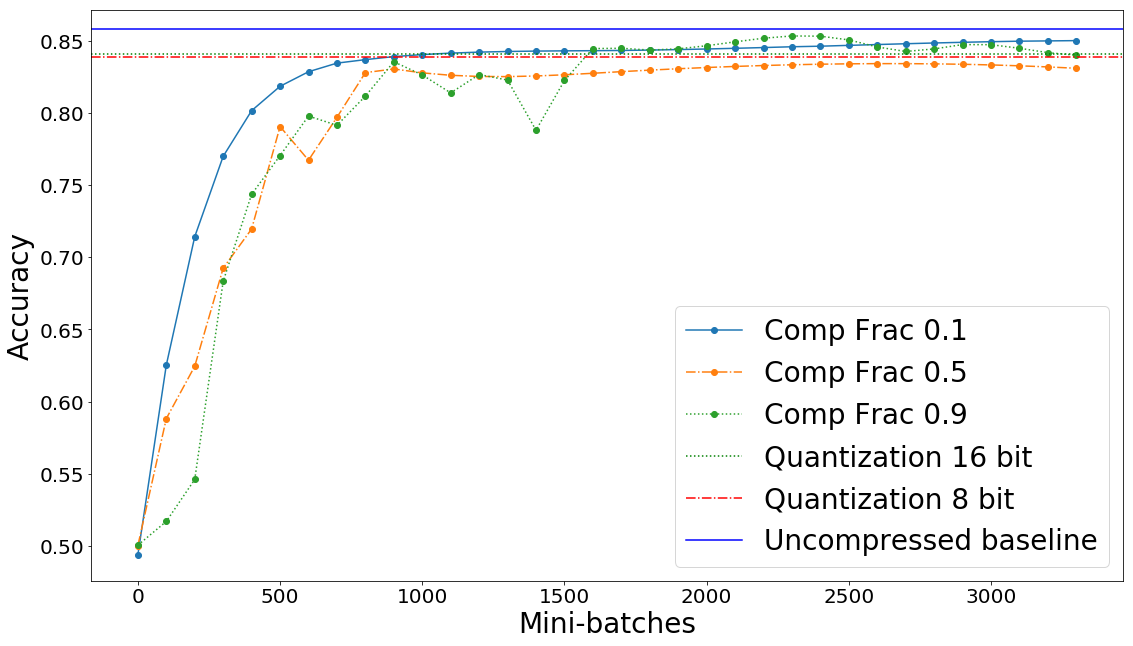
\includegraphics[height=60mm]{sst_lstm.png}
%			\captionof{figure}{\normalsize    LSTM model \label{plot:sst_lstm}}
%		\end{minipage}
%		\hfill
%		\begin{minipage}[b]{0.54\textwidth}
%			\centering 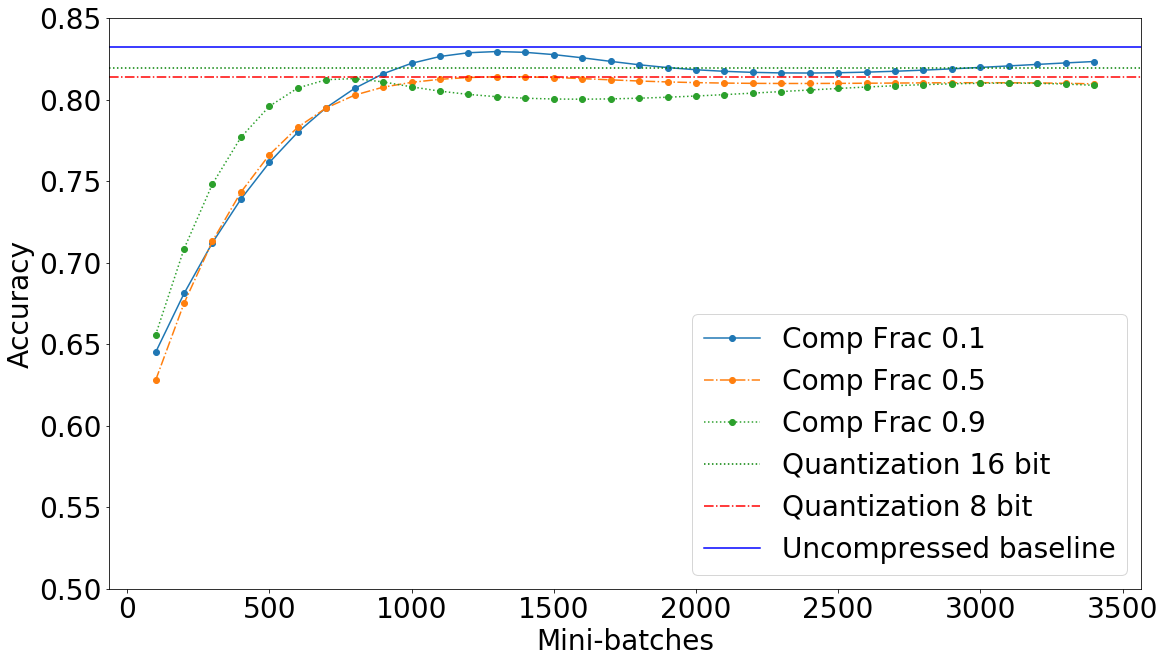
\includegraphics[height=60mm]{sst_dan.png}
%			\captionof{figure}{\normalsize    DAN model \label{plot:sst_dan}}
%		\end{minipage}
%	\end{minipage}
%       \caption{Dev set accuracy vs training mini batches for various compression percentages R for the SST2 datast}
%	%% \vspace{-0.4cm}
%\end{figure*}





%\begin{figure*}[htbp]
%	%% \vspace{-0.9cm}
%	\begin{minipage}{\textwidth}
%		\begin{minipage}[b]{0.54\textwidth}
%			\centering 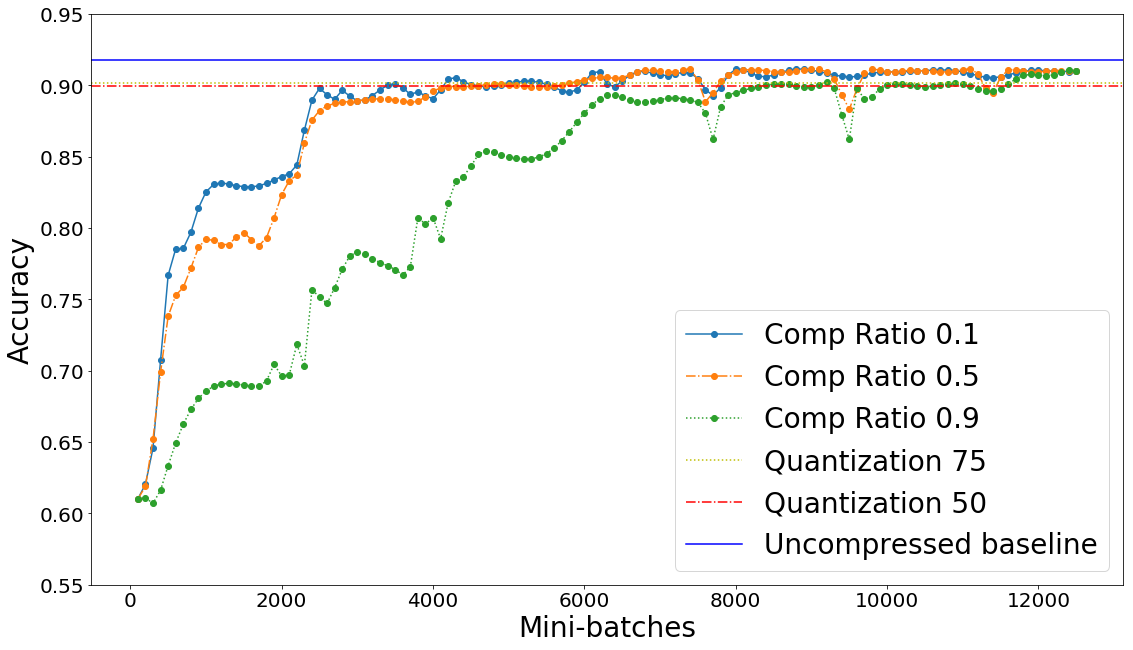
\includegraphics[height=60mm]{alexa_lstm.png}
%			\captionof{figure}{\normalsize    LSTM model \label{plot:intent_lstm}}
%		\end{minipage}
%		\hfill
%		\begin{minipage}[b]{0.54\textwidth}
%			\centering 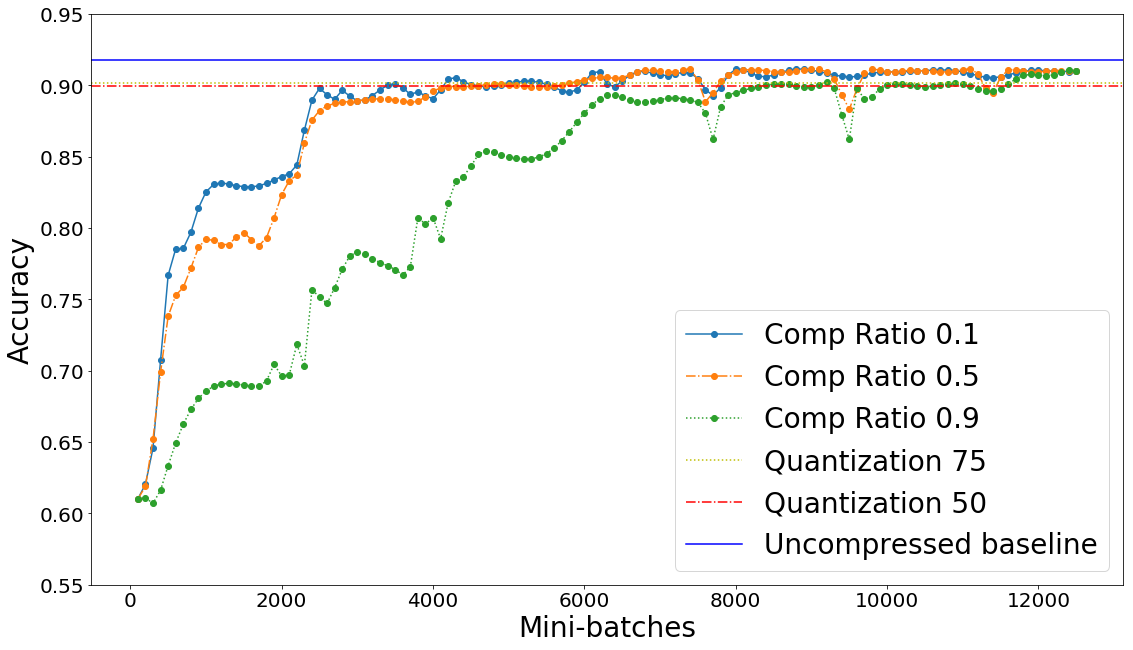
\includegraphics[height=60mm]{alexa_lstm.png}
%			\captionof{figure}{\normalsize    DAN model [ missing fig fix[ \label{plot:intent_dan}}
%		\end{minipage}
%	\end{minipage}
%        \caption{Accuracy vs mini batches for various compression ratios for the Intent datast}
%	%% \vspace{-0.4cm}
%\end{figure*}


%% %\iffalse
%%  \begin{figure}[htbp]
%% 	%\hspace{-1.7cm}
%% 	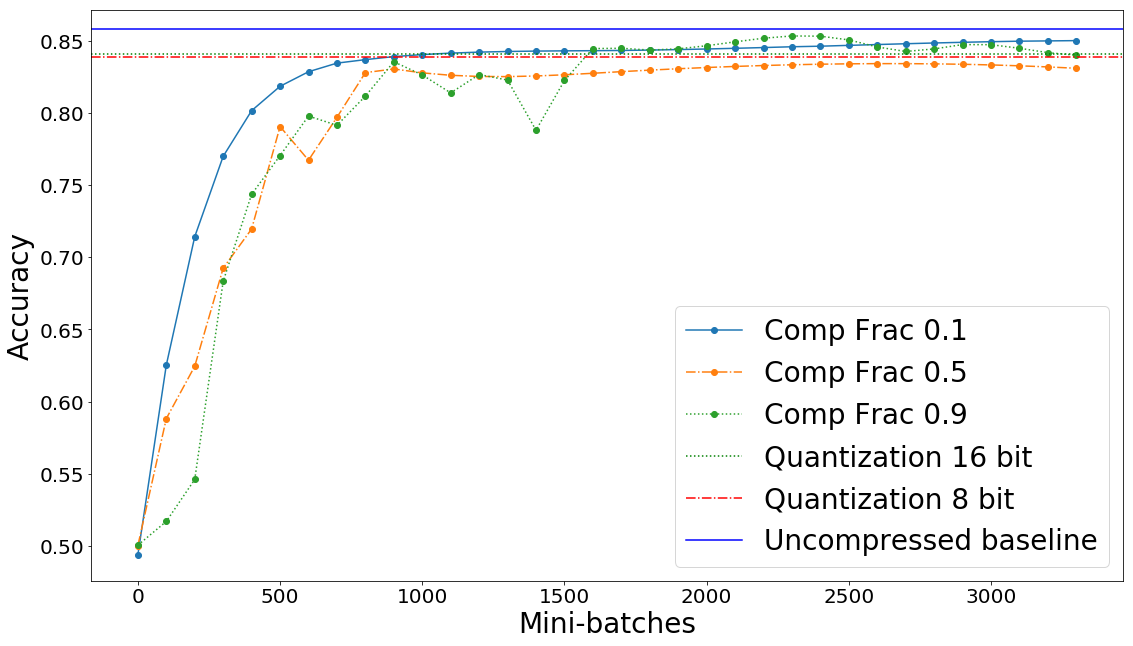
\includegraphics[height=52mm]{sst_lstm.png}
%% 	\caption{\normalsize Accuracy vs Epochs upon compressing the word embeddings with SST dataset with LSTM model\label{plot:sst_lstm}}
%% \end{figure}

%%  \begin{figure}[htbp]
%% 	%\hspace{-1.7cm}
%% 	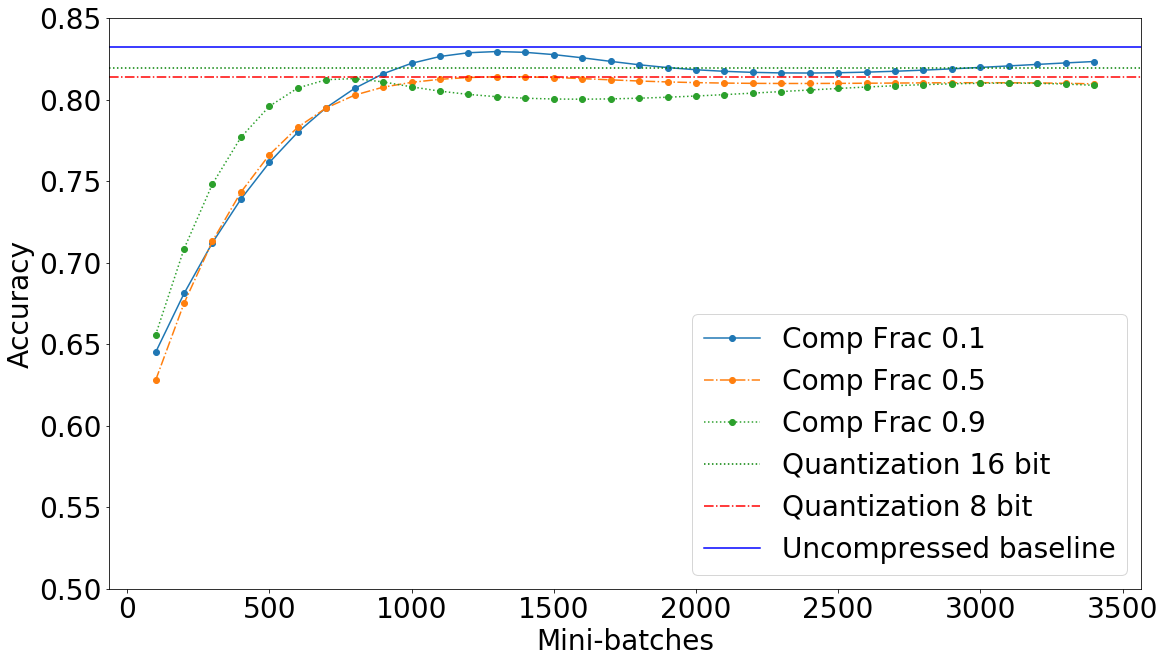
\includegraphics[height=52mm]{sst_dan.png}
%% 	\caption{\normalsize Accuracy vs Epochs upon compressing the word embeddings with SST dataset with the DAN model\label{plot:sst_dan}}
%% \end{figure}

 
%% \begin{figure}[htbp]
%% 	%\hspace{-0.5cm}
%% 	\includegraphics[height=52mm]{intent_lstm.png}
%% 	\caption{\normalsize Accuracy vs Epochs upon compressing the word embeddings on Intent Dataset with LSTM model\label{plot:intent_lstm}}
%% \end{figure}
%\fi

%% as the classifier. 
%% where we
%% use one hot
%% features and use 2 fully connected layers to predict the polarity which we then
%% compress at different compression ratios and fine tune.  We also repeat the
%% experiments with the word embeddings as an input feature and DANs~\cite{iyyer2015deep}
%% as the classifier. We plot the final fine tuned accuracy and compression ratio's in
%% Figure~\ref{fig:toy} and Figure~\ref{fig:state}. We compare them with the
%% quantized performance with 8 and 16 bit quantization as well.
%\subsection{Word Embeddings for Recipes}
